\documentclass{article}

\usepackage{graphicx, xcolor}
\usepackage{amsmath, amssymb}
\usepackage[colorlinks=true,allcolors=blue]{hyperref}

\usepackage[margin=1in]{geometry}

\def\hwtitle{Homework 4: Ordinary Differential Equations, Part \textsc{ii}}
\def\hwauthor{Caden Gobat}
\def\hwdate{\today}

\usepackage{fancyhdr}
\lhead{\hwauthor}
\chead{\hwtitle}
\rhead{\hwdate}
\lfoot{\hwauthor}
\cfoot{}
\rfoot{\thepage}
\renewcommand{\footrulewidth}{0.4pt}
\pagestyle{fancy}

\author{\hwauthor}
\title{\hwtitle}
\date{\hwdate}

\begin{document}

\maketitle
\thispagestyle{fancy}

\section{Introduction}

Last week we introduced Runge-Kutta methods for calculating numerical solutions to ODEs.

\section{Results}

\bigskip
\noindent{\bf Question 1}
\medskip

\begin{figure}[!h]
    \centering
    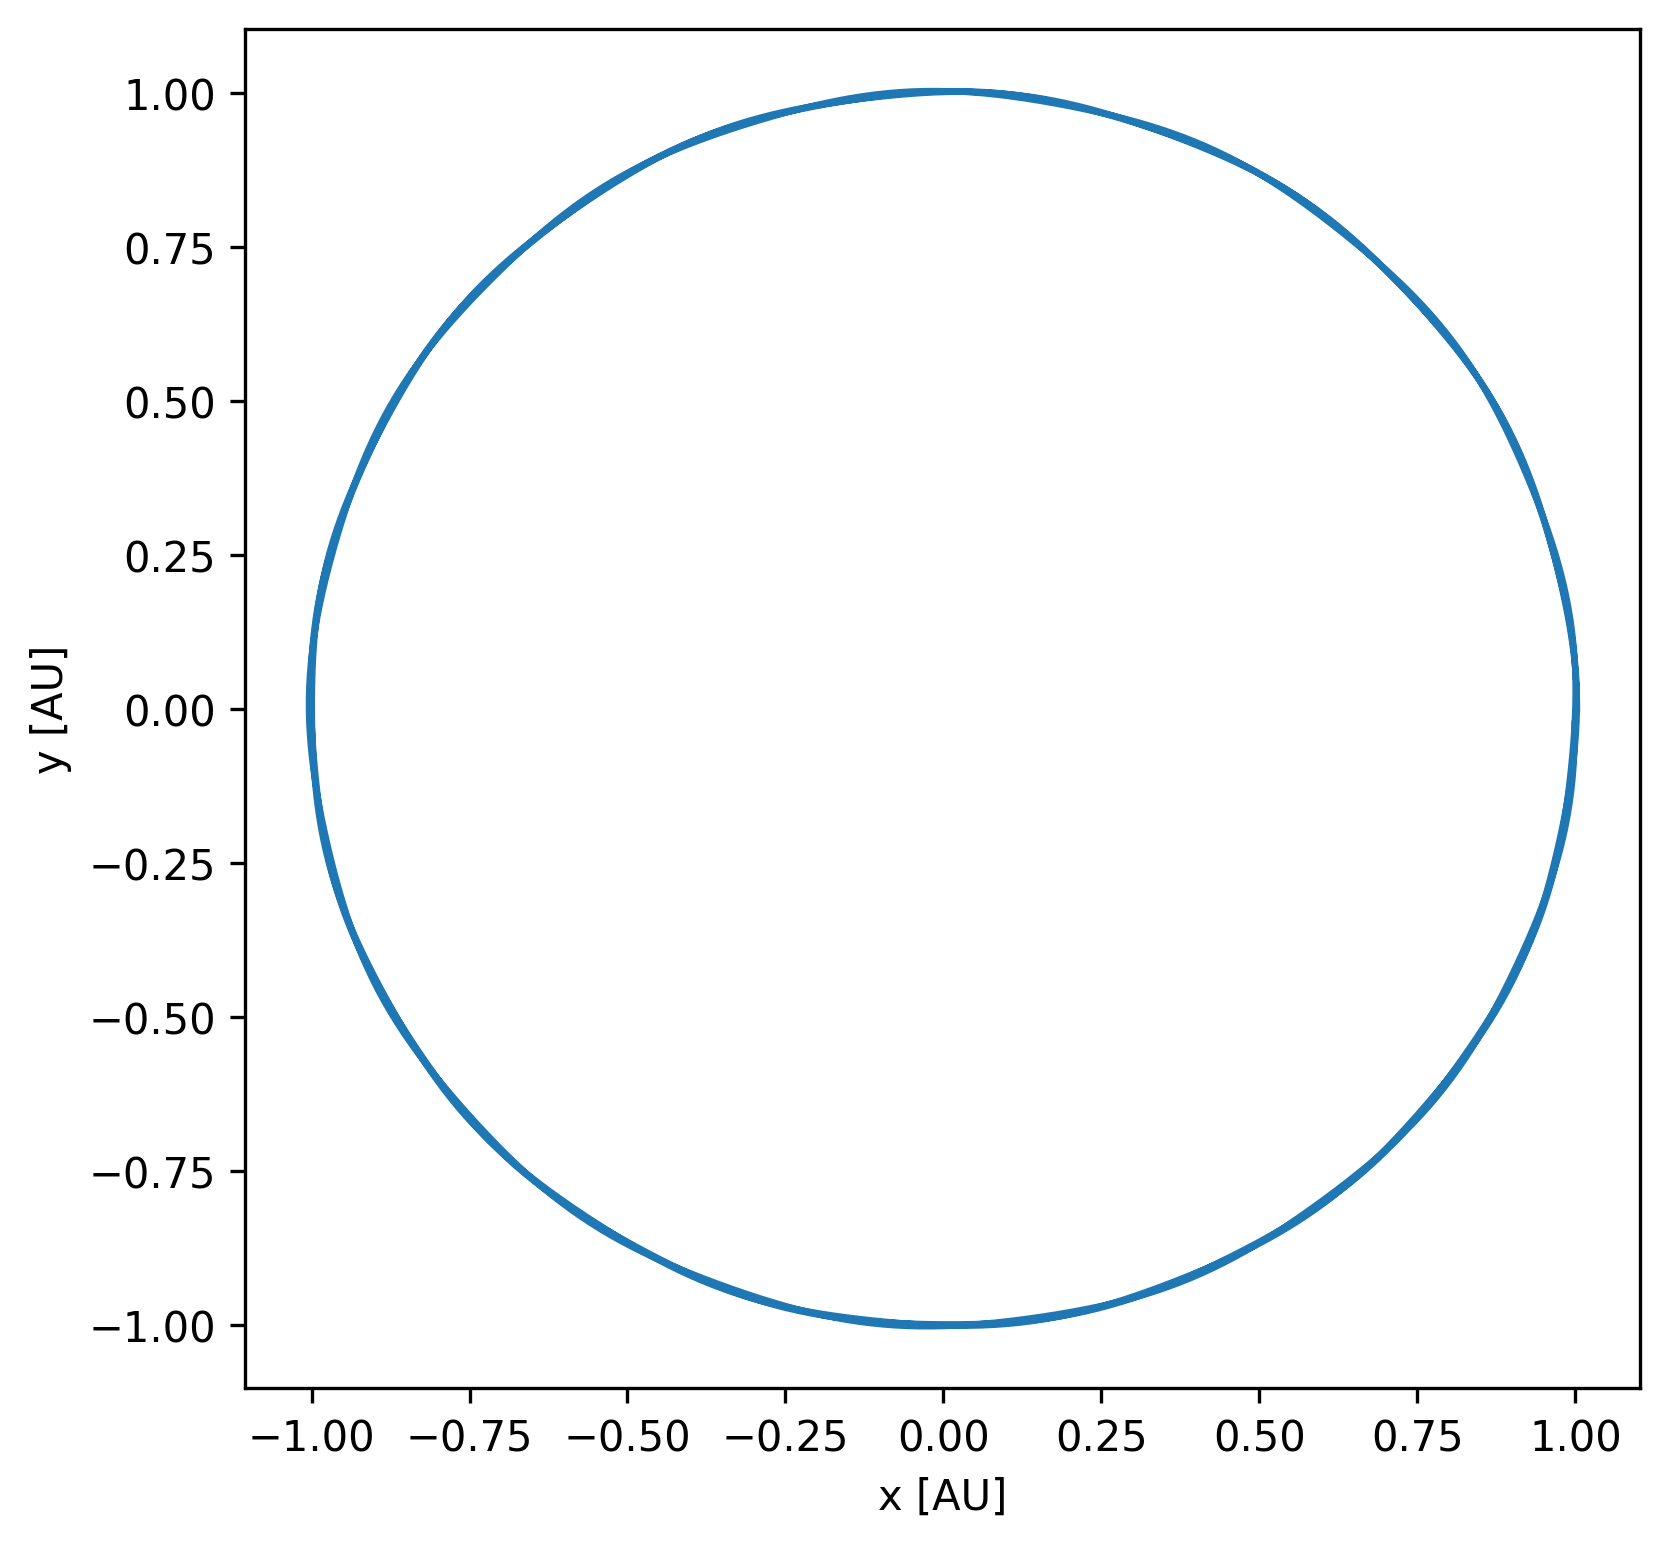
\includegraphics[width=3.5in]{homework4/1-1.png}
    \caption{Orbital trajectory over 3 years of the third (smallest) body in a 3-body system where $M_1=M_\odot$, $M_2=3\times10^{-6}M_\odot$, $M_3 = 3.7\times10^{-8}M_\odot$, $r_{12}=1$ AU, and $r_{23}= 0.0025$ AU. The calculated period of the second body (planet) is between 1.0013 and 1.0014 years.}
    \label{fig:1-1}
\end{figure}

\begin{figure}[!h]
    \centering
    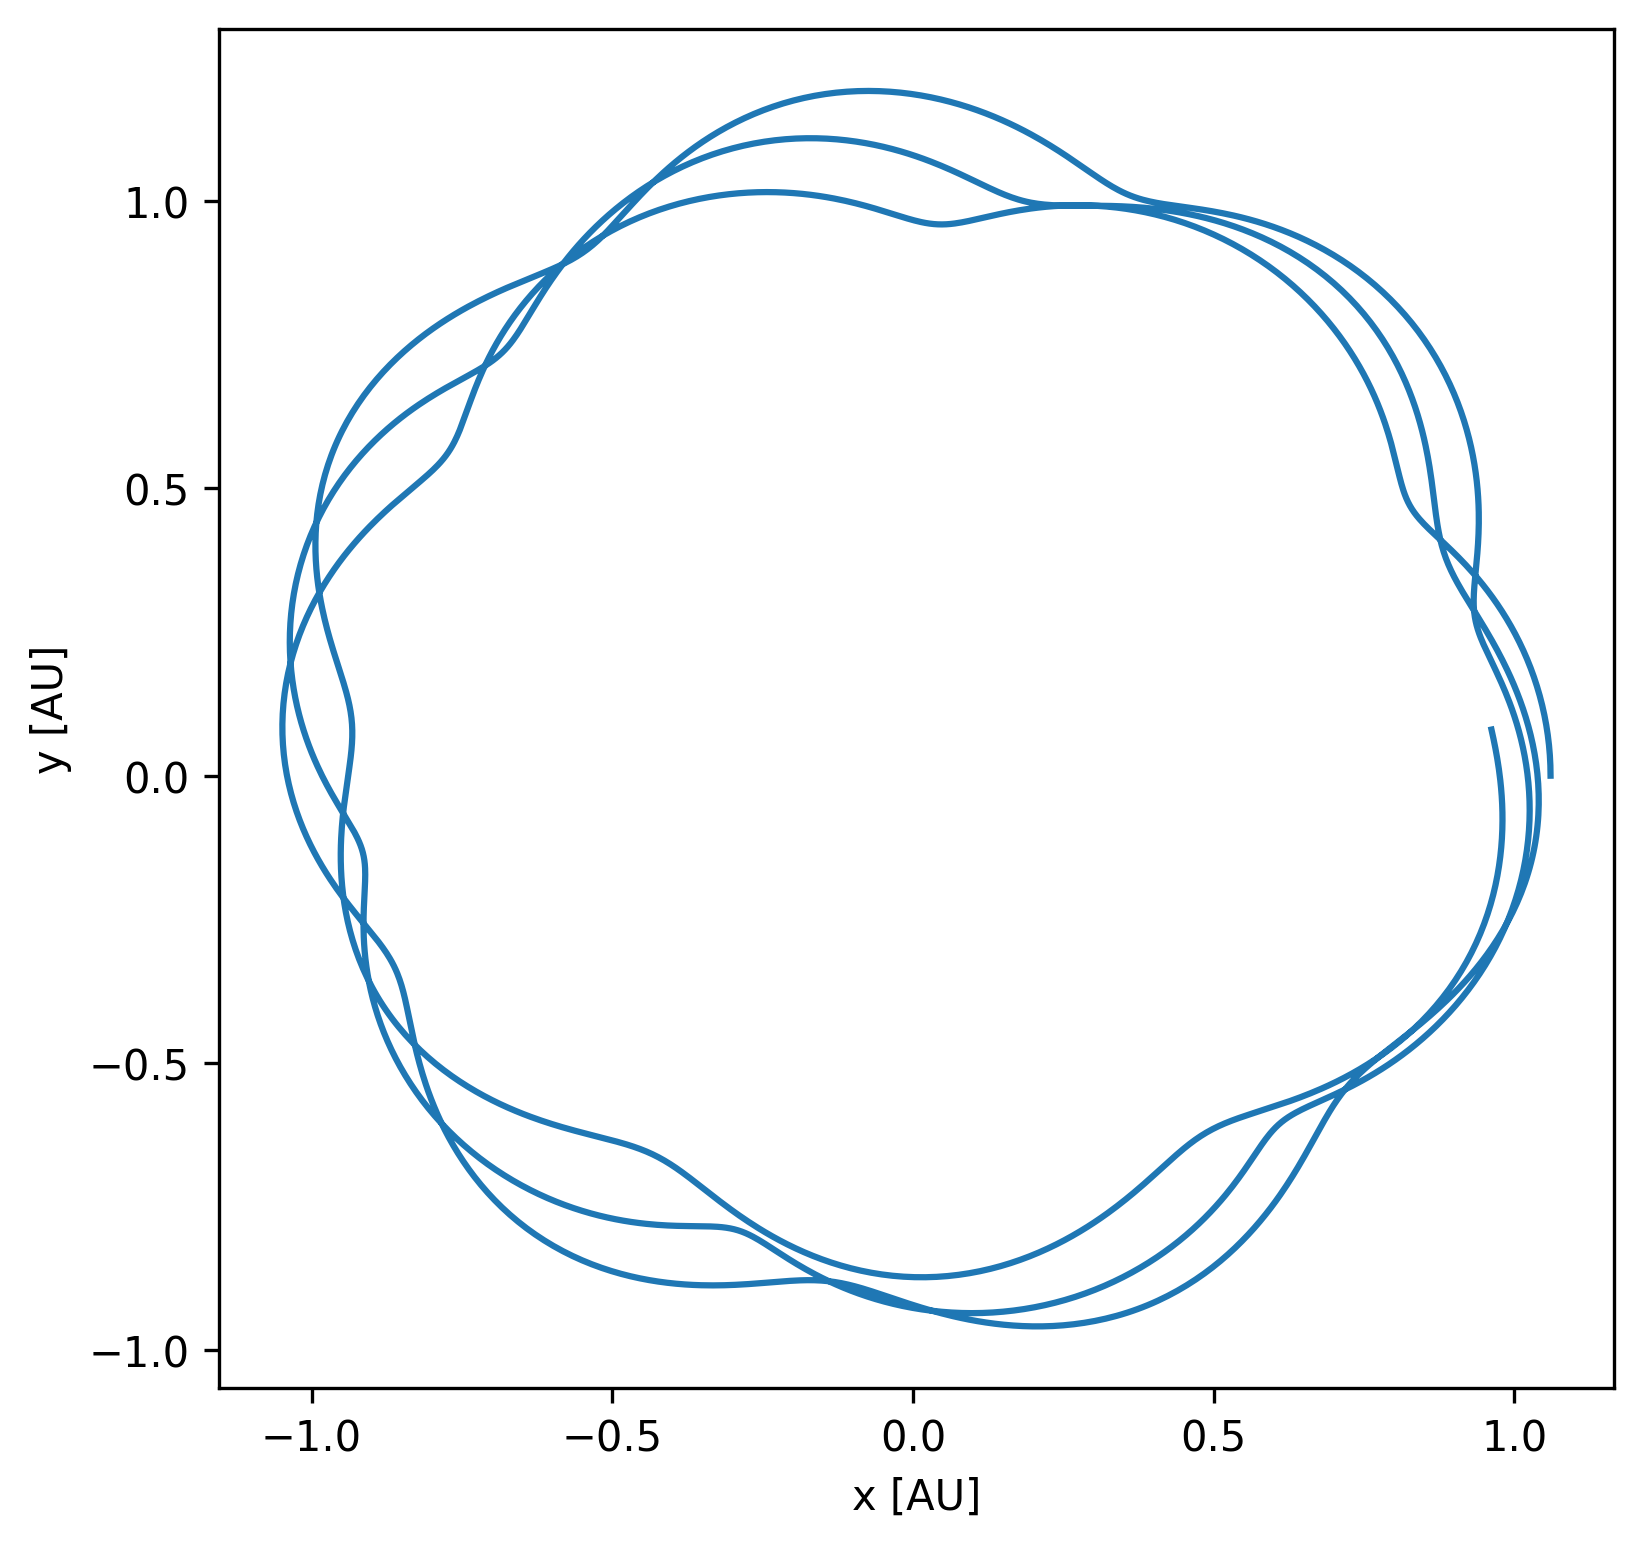
\includegraphics[width=3.5in]{homework4/1-2.png}
    \caption{Orbital trajectory over 3 years of the third (smallest) body in a 3-body system where $M_1=M_\odot$, $M_2=10^{-2}M_\odot$, $M_3 = 10^{-4}M_\odot$, $r_{12}=1$ AU, and $r_{23}= 0.0025$ AU. The calculated period of the second body (planet) is between 1.0188 and 1.0189 years.}
    \label{fig:1-2}
\end{figure}

\begin{figure}[!h]
    \centering
    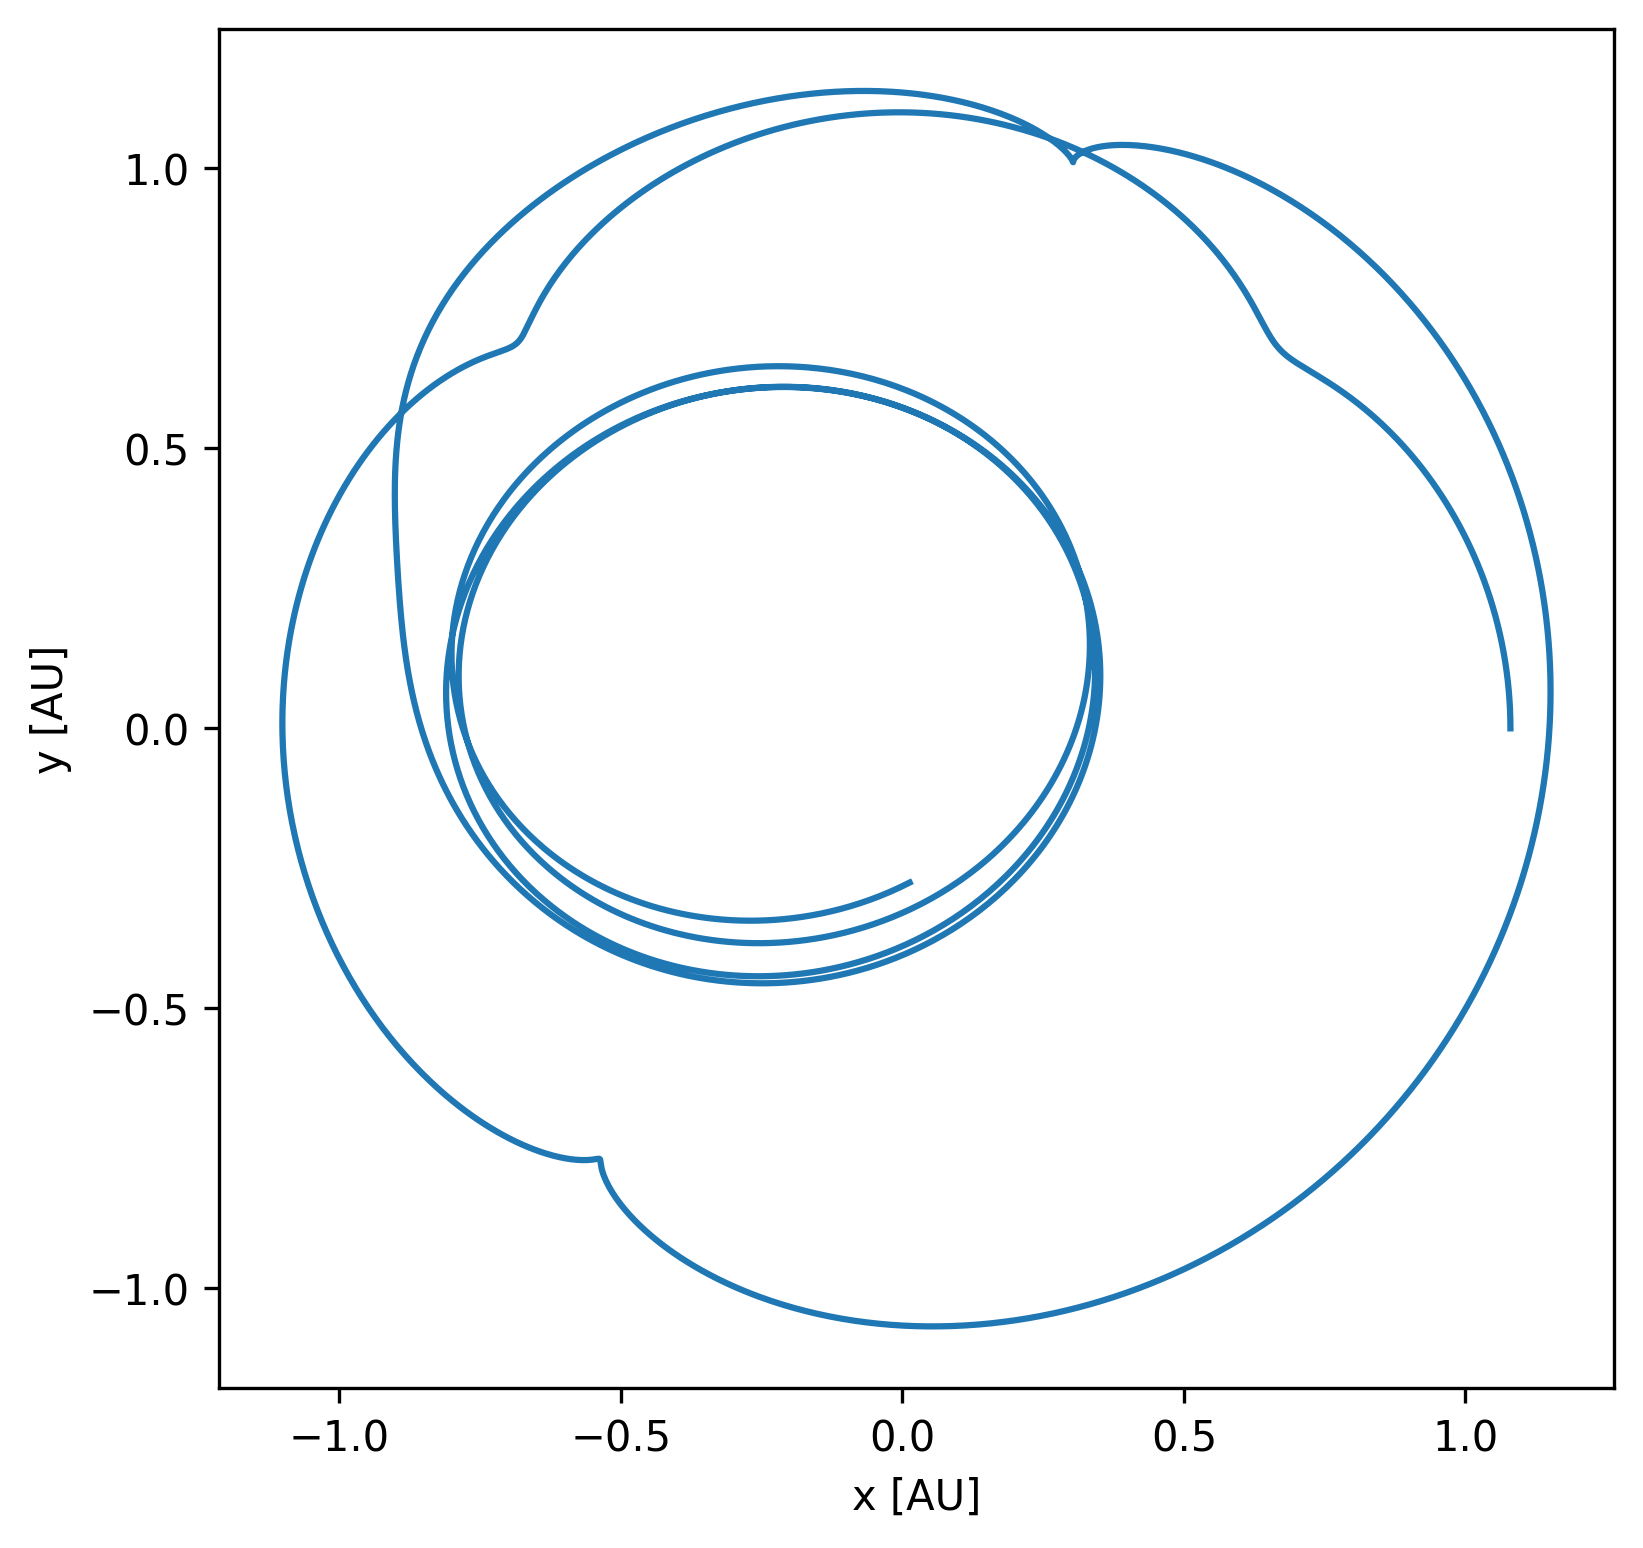
\includegraphics[width=3.5in]{homework4/1-3.png}
    \caption{Orbital trajectory over 3 years of the third (smallest) body in a 3-body system where $M_1=M_\odot$, $M_2=10^{-2}M_\odot$, $M_3 = 10^{-4}M_\odot$, $r_{12}=1$ AU, and $r_{23}= 0.08$ AU. The calculated period of the second body (planet) is between 1.0177 and 1.0178 years.}
    \label{fig:1-3}
\end{figure}

\begin{figure}[!h]
    \centering
    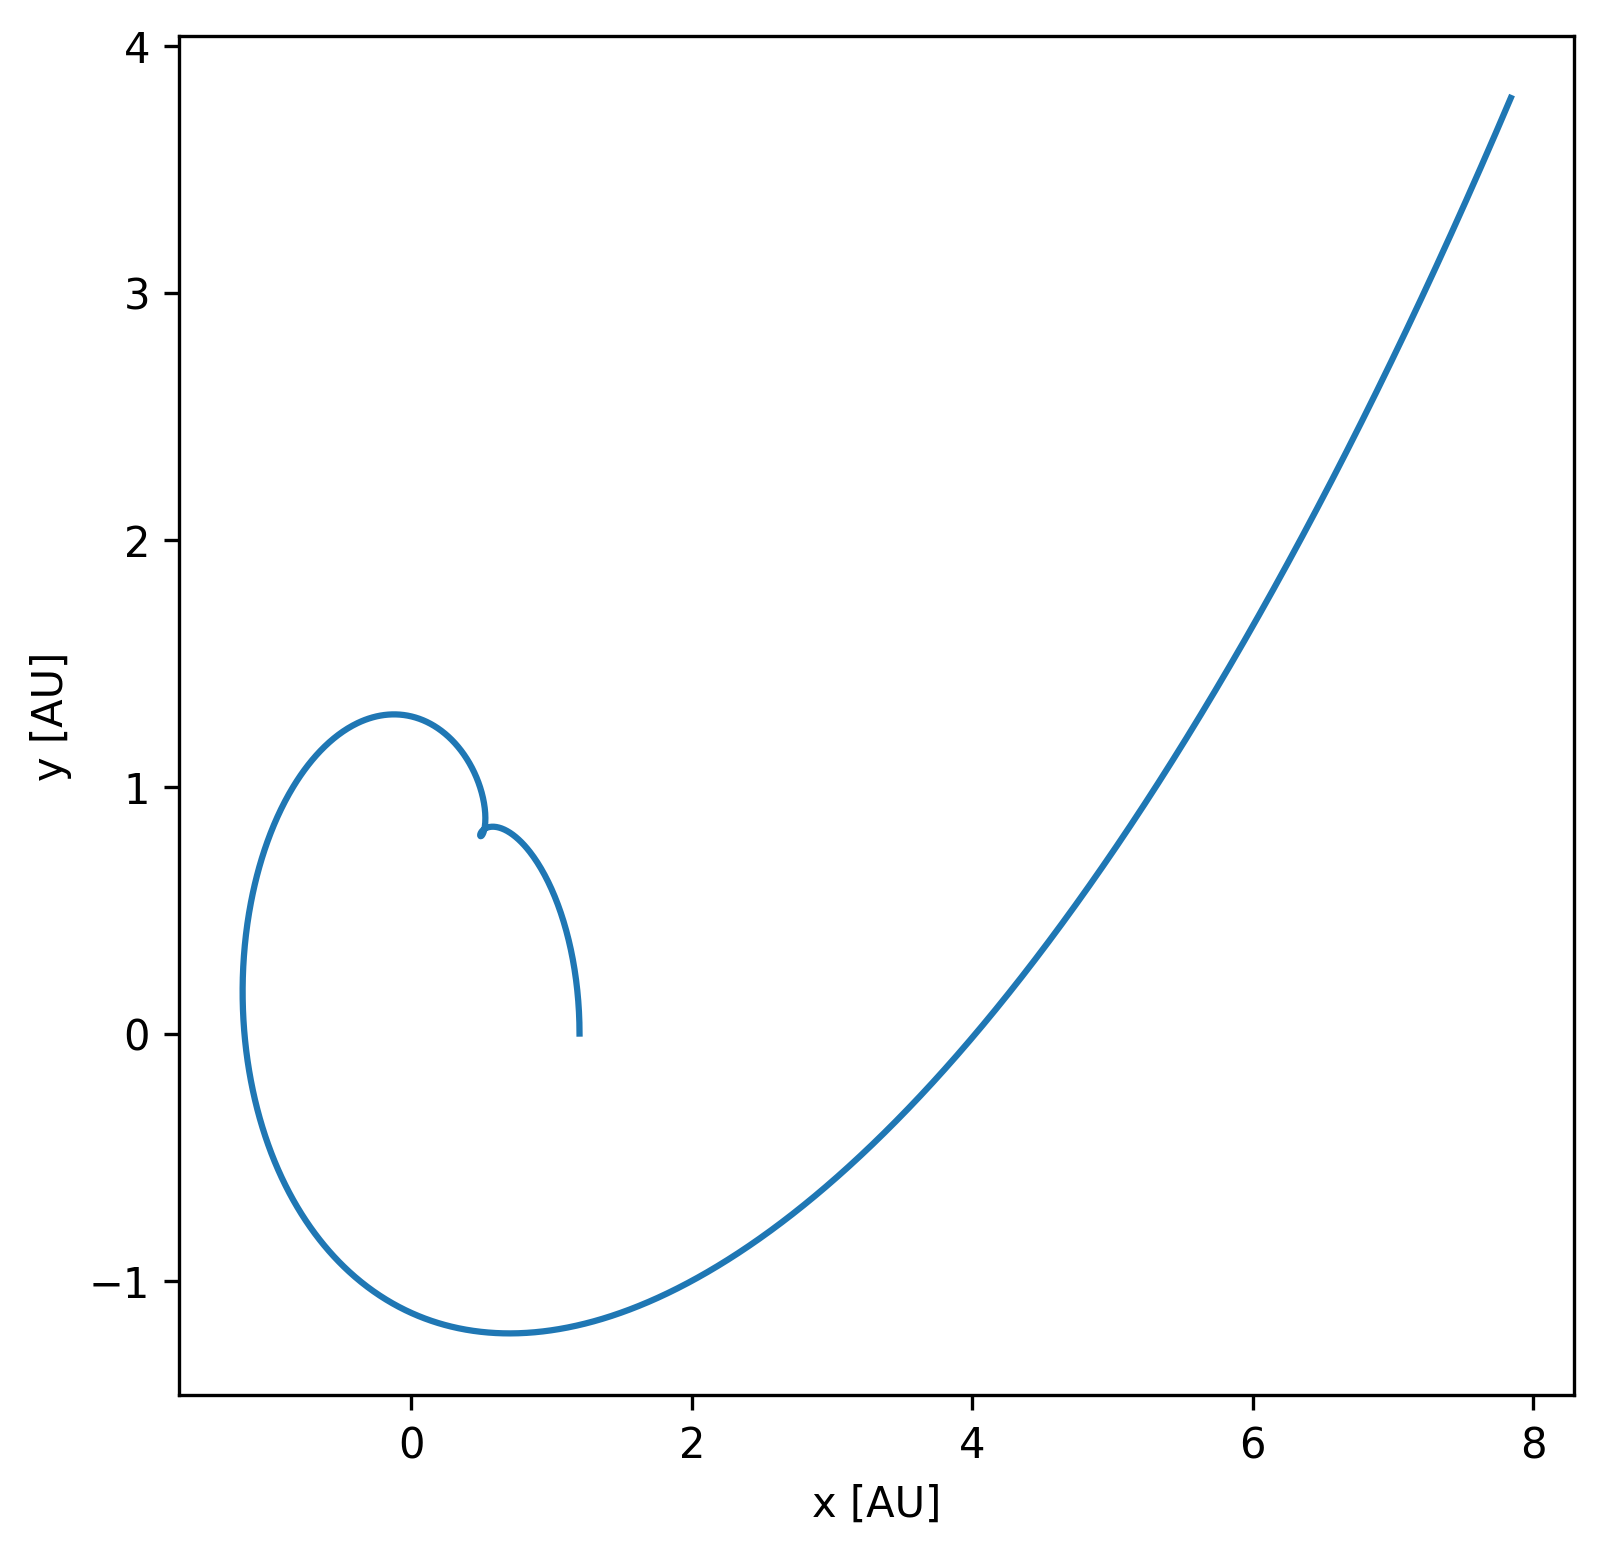
\includegraphics[width=3.5in]{homework4/1-4.png}
    \caption{Orbital trajectory over 3 years of the third (smallest) body in a 3-body system where $M_1=M_\odot$, $M_2=10^{-1}M_\odot$, $M_3 = 10^{-4}M_\odot$, $r_{12}=1$ AU, and $r_{23}= 0.2$ AU. The calculated period of the second body (planet) is between 1.0192 and 1.0193 years.}
    \label{fig:1-4}
\end{figure}

The period for the planet in each case is $\ \sim 1$ year because the initial velocities are specified such that a circular orbit will complete 1 revolution in 1 year. Changing $dt$ has little effect on these results, as the orbits for the planet are still mostly circular or elliptical, and so there is not as much accuracy to be lost in small, nuanced movements as is the case for the third, smallest body.

\section{Conclusions}

As compared to previous assignments, I had a few more technical difficulties this time around. At first my \texttt{C} code was not functioning properly at all, and I had to scale back on some of the generalizability that I had tried to implement during the debugging process.

Additionally, the requested timestep of $dt=10^{-6}$ years is extremely computationally demanding, especially when the time domain spans 8 or 12 years. I found myself sitting idle for long periods of time simply waiting for my code to finish execution, before even knowing if the results were good or not. Additionally, the simulation results and output are at least 1--2 GB in size for some of the time domains required in this assignment. I compared the shapes of the orbits using $dt=10^{-5}$ years and $dt=10^{-6}$ years and found only minimal differences, so I hesitate to say that the marginally increased accuracy afforded by the smaller time step is worth the increased computational time.

\end{document}
